
%%%%%%%%%%%%%%%%%%%%%%%%%%%%%%%%%%%%%%%%%%%%%%%%%%%%%%%%%%
%%%%%%%%%%%%%%%%%%%%    宽高比设置    %%%%%%%%%%%%%%%%%%%%%%
%%%%%%%%%%%%%%%%%%%%%%%%%%%%%%%%%%%%%%%%%%%%%%%%%%%%%%%%%%
%% 4:3
% \documentclass[aspectratio=43]{ahu-slide}
% \newlength{\pheight}
% \setlength{\pheight}{0.36\linewidth}    % 43
%% 16:10
% \documentclass[aspectratio=1610]{ahu-slide}
% \newlength{\pheight}
% \setlength{\pheight}{0.29\linewidth}    % 1610
%% 16:9
\documentclass[aspectratio=169]{ahu-slide}
\newlength{\pheight}
\setlength{\pheight}{0.25\linewidth} 

%%%%%%%%%%%%%%%%%%%%%%%%%%%%%%%%%%%%%%%%%%%%%%%%%%%%%%%%%%
%%%%%%%% AHU Undergraduates Thesis Slide Template %%%%%%%%
%%%%%%%%%%%%%%%%%%%%%%%%%%%%%%%%%%%%%%%%%%%%%%%%%%%%%%%%%%

\usepackage{multirow}		% 表格
\usepackage{amssymb}
\usepackage{amsmath} 

\usepackage{setspace}       % 行间距


%%%%%%%%%%%%%%%%%%%%%%%%%%%%%%%%%%%%%%%%%%%%%%%%%%%%%%%%%%
%%%%%%%%               时间线绘图相关               %%%%%%%%
%%%%%%%%%%%%%%%%%%%%%%%%%%%%%%%%%%%%%%%%%%%%%%%%%%%%%%%%%%
\usepackage[usenames,dvipsnames]{xcolor}
\usetikzlibrary{calc, arrows.meta, intersections, patterns, positioning, shapes.misc, fadings, through, decorations.pathreplacing}
% 颜色
\definecolor{MidnightBlue}{HTML}{006795}
\definecolor{RedOrange}{HTML}{F26035}
\definecolor{Plum}{HTML}{92268F}
\definecolor{Dandelion}{HTML}{00CD00}


% 取消注释可自定义颜色
% 深蓝色示例
% \definecolor{ahublue}{RGB}{0,68,170}
% \definecolor{ahulightblue}{RGB}{200,222,255}
% 橙色示例
% \definecolor{ahublue}{RGB}{249,138,0}
% \definecolor{ahulightblue}{RGB}{255,231,200}
% 粉色示例
% \definecolor{ahublue}{RGB}{219,115,188}
% \definecolor{ahulightblue}{RGB}{255,206,239}

% 取消注释可自定义字体(例如使用 macOS 下更好看的字体)
% \setsansfont{SF Pro}
% \setCJKsansfont{PingFang SC}

% 浅色主题 / 深色主题(注释即为浅色)
\dark

% 底部控制放映的导航条(取消注释则不显示)
\nav

% 封面的题目
\title{答辩题目}

% 答辩人
\author{xxx}

% 指导教师
\teacher{xxx}

% 答辩时间
\pubdate{2025-05-15}

\begin{document}

% 封面
\maketitle

% 目录页
\begin{frame}{目录}
    \tableofcontents
\end{frame}

% 第一部分 转场
\ahusection{研究背景与意义}{Research background}

\begin{frame}{图文举例}
    \textbf{单目标跟踪(SOT):}给定任意目标的初始状态(位置和大小),预测目标在后续帧中的状态。
    在军事侦查、安防监控、智能交通等领域都有广泛的运用。

    \textbf{RGBT视觉跟踪:}在SOT基础上,引入热红外模态,克服可见光模态在雨雪雾等恶劣天气和极端光照下失效的问题。\par

    \begin{figure}
        \centering
        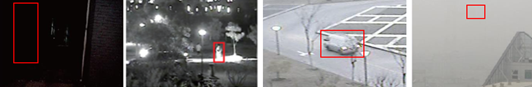
\includegraphics[width=1\linewidth]{paper_figs/成像相关的挑战.png}
    \end{figure}
\end{frame}


\begin{frame}{双栏举例}

    \vskip -0.5cm
    \begin{table}
        \resizebox{\linewidth}{!}{
        \begin{tabular}{c|c|c}
            \hline
             & \textbf{可见光(RGB)} & \textbf{热红外(TIR)}\\
             \hline
           \textbf{优势} & 分辨率高,纹理清晰色彩信息丰富 & 基本不受光照和雾霾因素影响 \\
           \hline
           \textbf{劣势} & 光照敏感,对雾霾等穿透能力差 & 纹理细节弱,对玻璃等穿透能力差 \\
           \hline
        \end{tabular}
        }
    \end{table}
    
    \vskip -0.3cm
    \begin{columns}
        \column{0.03\textwidth}
        \column{0.36\textwidth}
        \begin{figure}
            \centering
            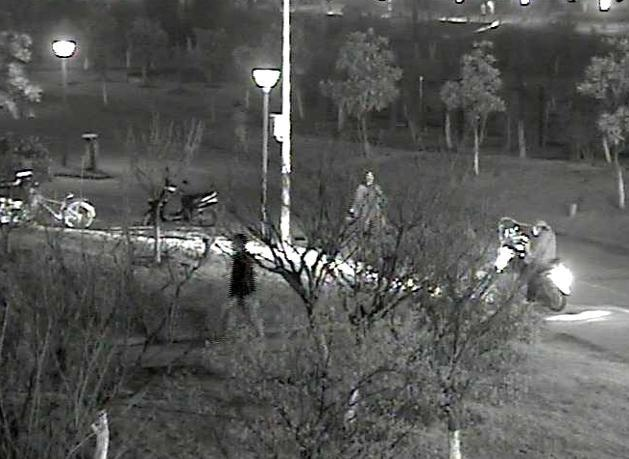
\includegraphics[height=0.7\pheight]{paper_figs/RGB_1.jpg}
        \end{figure}
        \vskip -0.5cm
        \begin{figure}
            \centering
            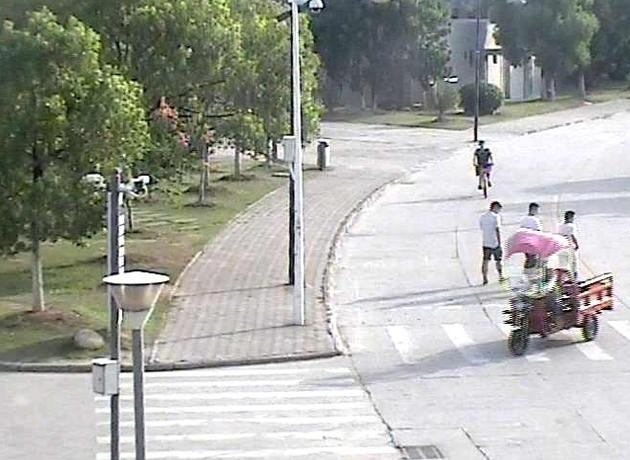
\includegraphics[height=0.7\pheight]{paper_figs/RGB_2.jpg}
        \end{figure}
    
        \column{0.36\textwidth}
        \begin{figure}
            \centering
            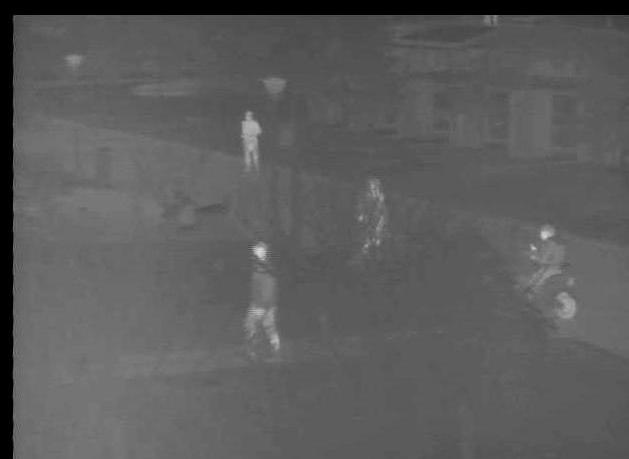
\includegraphics[height=0.7\pheight]{paper_figs/TIR_1.jpg}
        \end{figure}
        \vskip -0.5cm
        \begin{figure}
            \centering
            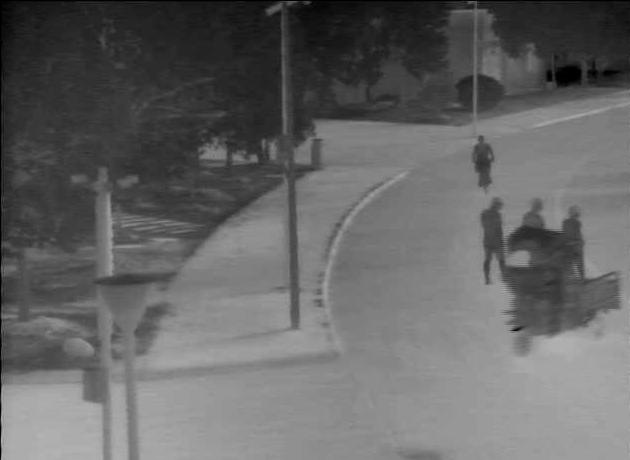
\includegraphics[height=0.7\pheight]{paper_figs/TIR_2.jpg}
        \end{figure}
    \end{columns}

\end{frame}


\ahusection{国内外研究现状}{Related research}

\begin{frame}{时间线绘图示例}

%%%%%%%%%%%%%%%%%%%%%%%%%%%%%%%%%%%%% 4:3
% \begin{columns}

% \column{1.1\linewidth}
% \tikzstyle{descript} = [text = black,align=center, minimum height=1.6cm, align=center, outer sep=0pt,font = \footnotesize]
% \tikzstyle{activity} =[align=center,outer sep=1pt]
% 	\begin{tikzpicture}[very thick, black]
% 		\small
% 		%% Coordinates
%         %% 4:3
% 		\coordinate (O) at (-2,0);
% 		\coordinate (P16) at (0,0);
% 		\coordinate (P21) at (3,0);
% 		\coordinate (P22) at (5,0);
% 		\coordinate (P23) at (7,0);
% 		\coordinate (P24) at (9,0);
% 		\coordinate (F) at (10,0);
% 		\coordinate (boxh) at (0,0.7);    % 色块高度
		
% 		%% Main Events
%         \shade[left color=MidnightBlue!5, right color=MidnightBlue!20] rectangle (O) -- (P16) -- ($(P16)+(boxh)$) -- ($(O)+(boxh)$);
% 		\fill[color=RedOrange!20] rectangle (P16) -- (P21) -- ($(P21)+(boxh)$) -- ($(P16)+(boxh)$);
% 		\fill[color=Plum!20] rectangle (P21) -- (P23) -- ($(P23)+(boxh)$) -- ($(P21)+(boxh)$);
% 		\shade[left color=Dandelion, right color=white] rectangle (P23) -- (F) -- ($(F)+(boxh)$) -- ($(P23)+(boxh)$);
% 		\draw ($(P16)+(-1,0.35)$) node[activity,MidnightBlue] {传统方法};
% 		\draw ($(P21)+(-1.5,0.35)$) node[activity,RedOrange] {卷积};
% 		\draw ($(P23)+(-2,0.35)$)  node[activity,Plum] {卷积+Trans};
% 		\draw ($(F)+(-1.5,0.35)$)  node[activity,Dandelion] {Trans};
		
% 		%% Description
% 		\node[descript,fill=RedOrange!15,text=RedOrange](DMDNet) at ($(P16)+(-0.4,2.1)$) {
% 			\begin{minipage}{0.25\textwidth}
% 				\centering
% 				\textbf{MDNet提出}\\
% 				在线更新性能好\\
% 				{\tiny CAT、CMPP、DMCNet...}
% 			\end{minipage}};
		
% 		\node[descript,fill=RedOrange!15,text=RedOrange](DSiamFC) at ($(P16)+(-0.1,-2)$) {
% 			\begin{minipage}{0.25\textwidth}
% 				\centering
% 				\textbf{SiamFC提出}\\
% 				离线训练效率高\\
% 				 {\tiny SiamCDA、SiamVIFN...}
% 			\end{minipage}};
		
% 		\node[descript,fill=RedOrange!15,text=RedOrange](DCAT) at ($(P21)+(0.2,2.1)$) {
% 			\begin{minipage}{0.25\textwidth}
% 				\centering
% 				\textbf{CAT提出}\\
% 				属性解耦\\
%                 {\tiny ADRNet、APFNet、CAT++...}
% 			\end{minipage}};
            
% 		\node[descript,fill=Plum!15,text=Plum](DTransT) at ($(P22)+(-1.2,-2)$) {
% 			\begin{minipage}{0.25\textwidth}
% 				\centering
% 				\textbf{TransT提出}\\
% 				Trans替代特征融合\\
%                 {\tiny APFNet、Proformer、MIRNet...}
% 			\end{minipage}};
		
% 		\node[descript,fill=Plum!15,text=Plum](DOSTrack) at ($(P23)+(-0.3,2.1)$) {
% 			\begin{minipage}{0.25\textwidth}
% 				\centering
% 				\textbf{OSTrack提出}\\
% 				完全使用Trans\\
% 				{\tiny TBSI、ViPT、BAT...}
% 			\end{minipage}};
		
		
% 		\node[descript,fill=Dandelion!15,text=Dandelion](DViPT) at ($(P23)+(0.3,-2)$) {%
% 			\begin{minipage}{0.25\textwidth}
% 				\centering
% 				\textbf{ViPT提出}\\
% 				高效微调\\
%                 {\tiny BAT、SDSTrack...}
% 			\end{minipage}};
		
% 		%% Arrows
% 		\path[->,color=RedOrange] ($(P16)+(0.1,0.6)$) edge [out=90, in=-50]  ($(DMDNet)-(0,0.9)$);
% 		\path[->,color=RedOrange] ($(P16)+(0.3,-0.1)$) edge [out=-90, in=110]  ($(DSiamFC)+(0,0.9)$);
% 		\path[->,color=RedOrange] ($(P16)+(1.5,0.6)$) edge [out=80, in=-100]  ($(DCAT)-(0,0.9)$);
% 		\path[->,color=Plum] ($(P21)+(0.4,-0.1)$) edge [out=-70, in=100]  ($(DTransT)+(0,0.9)$);
% 		\path[->,color=Plum] ($(P22)+(0.8,0.6)$) edge [out=60, in=-120]  ($(DOSTrack)-(0,0.9)$);
% 		\path[->,color=Dandelion]($(P23)+(0.5,-0.1)$)  edge [out=-70, in=90]  ($(DViPT)+(0,0.9)$);
		
% 		%% Arrow
% 		\draw[->] (O) -- (F);
% 		%% Ticks
% 		\foreach \x in {0,3,5,7,9}
% 		\draw(\x cm,3pt) -- (\x cm,-3pt);
% 		%% Labels
% 		\foreach \i \j in {0/2016,3/2021,5/2022,7/2023,9/2024}{
% 			\draw (\i,0) node[below=3pt] {\j} ;
% 		}
% 	\end{tikzpicture}
    
% \end{columns}

%%%%%%%%%%%%%%%%%%%%%%%%%%%%%%%%%%%% 16:10

\vskip 0.1cm
\begin{columns}
\column{1.1\linewidth}
\tikzstyle{descript} = [text = black,align=center, minimum height=1.6cm, align=center, outer sep=0pt,font = \footnotesize]
\tikzstyle{activity} =[align=center,outer sep=1pt]
	\begin{tikzpicture}[very thick, black]
		\small
		%% Coordinates
        %% 4:3
		\coordinate (O) at (-2,0);
		\coordinate (P16) at (0,0);
		\coordinate (P21) at (3.5,0);
		\coordinate (P22) at (6,0);
		\coordinate (P23) at (8.5,0);
		\coordinate (P24) at (11,0);
		\coordinate (F) at (12.5,0);
		\coordinate (boxh) at (0,0.7);    % 色块高度
		
		%% Main Events
        \shade[left color=MidnightBlue!5, right color=MidnightBlue!20] rectangle (O) -- (P16) -- ($(P16)+(boxh)$) -- ($(O)+(boxh)$);
		\fill[color=RedOrange!20] rectangle (P16) -- (P21) -- ($(P21)+(boxh)$) -- ($(P16)+(boxh)$);
		\fill[color=Plum!20] rectangle (P21) -- (P23) -- ($(P23)+(boxh)$) -- ($(P21)+(boxh)$);
		\shade[left color=Dandelion, right color=white] rectangle (P23) -- (F) -- ($(F)+(boxh)$) -- ($(P23)+(boxh)$);
		\draw ($(P16)+(-1,0.35)$) node[activity,MidnightBlue] {传统方法};
		\draw ($(P21)+(-1.9,0.35)$) node[activity,RedOrange] {卷积};
		\draw ($(P23)+(-2.5,0.35)$)  node[activity,Plum] {卷积+Trans};
		\draw ($(F)+(-2,0.35)$)  node[activity,Dandelion] {Trans};
		
		%% Description
		\node[descript,fill=RedOrange!15,text=RedOrange](DMDNet) at ($(P16)+(-0.4,2.1)$) {
			\begin{minipage}{0.25\textwidth}
				\centering
				\textbf{MDNet提出}\\
				在线更新性能好\\
				{\tiny CAT、CMPP、DMCNet...}
			\end{minipage}};
		
		\node[descript,fill=RedOrange!15,text=RedOrange](DSiamFC) at ($(P16)+(-0.1,-2)$) {
			\begin{minipage}{0.25\textwidth}
				\centering
				\textbf{SiamFC提出}\\
				离线训练效率高\\
				 {\tiny SiamCDA、SiamVIFN...}
			\end{minipage}};
		
		\node[descript,fill=RedOrange!15,text=RedOrange](DCAT) at ($(P21)+(0.8,2.1)$) {
			\begin{minipage}{0.25\textwidth}
				\centering
				\textbf{CAT提出}\\
				基于属性解耦的融合策略\\
                {\tiny ADRNet、APFNet、CAT++...}
			\end{minipage}};
            
		\node[descript,fill=Plum!15,text=Plum](DTransT) at ($(P22)+(-1.2,-2)$) {
			\begin{minipage}{0.25\textwidth}
				\centering
				\textbf{TransT提出}\\
				Trans替代特征融合\\
                {\tiny APFNet、Proformer、MIRNet...}
			\end{minipage}};
		
		\node[descript,fill=Plum!15,text=Plum](DOSTrack) at ($(P23)+(0.3,2.1)$) {
			\begin{minipage}{0.25\textwidth}
				\centering
				\textbf{OSTrack提出}\\
				完全使用Trans\\
				{\tiny TBSI、ViPT、BAT...}
			\end{minipage}};
		
		
		\node[descript,fill=Dandelion!15,text=Dandelion](DViPT) at ($(P23)+(0.7,-2)$) {%
			\begin{minipage}{0.25\textwidth}
				\centering
				\textbf{ViPT提出}\\
				高效微调\\
                {\tiny BAT、SDSTrack...}
			\end{minipage}};
		
		%% Arrows
		\path[->,color=RedOrange] ($(P16)+(0.1,0.6)$) edge [out=90, in=-50]  ($(DMDNet)-(0,0.9)$);
		\path[->,color=RedOrange] ($(P16)+(0.3,-0.1)$) edge [out=-90, in=110]  ($(DSiamFC)+(0,0.9)$);
		\path[->,color=RedOrange] ($(P16)+(1.5,0.6)$) edge [out=80, in=-100]  ($(DCAT)-(0,0.9)$);
		\path[->,color=Plum] ($(P21)+(0.4,-0.1)$) edge [out=-70, in=100]  ($(DTransT)+(0,0.9)$);
		\path[->,color=Plum] ($(P22)+(0.8,0.6)$) edge [out=60, in=-120]  ($(DOSTrack)-(0,0.9)$);
		\path[->,color=Dandelion]($(P23)+(0.5,-0.1)$)  edge [out=-70, in=90]  ($(DViPT)+(0,0.9)$);
		
		%% Arrow
		\draw[->] (O) -- (F);
		%% Ticks
		\foreach \x in {0,3.5,6,8.5,11}
		\draw(\x cm,3pt) -- (\x cm,-3pt);
		%% Labels
		\foreach \i \j in {0/2016,3.5/2021,6/2022,8.5/2023,11/2024}{
			\draw (\i,0) node[below=3pt] {\j} ;
		}
	\end{tikzpicture}
    
\end{columns}

\begin{enumerate}
    \item 按照融合阶段划分,特征融合是主流
    \item 按照基线跟踪器看,采用Vision Transformer是趋势
\end{enumerate}
\end{frame}



\begin{frame}{公式举例}
\begin{block}{风格损失}
提取分布信息,作为风格特征:
$\mu^{s(l)} = \frac{1}{N} \sum_{n=1}^{N} f^{l(n)}, \sigma^{s(l)} = \sqrt{\frac{1}{N} \sum_{n=1}^{N} (f^{l(n)} - \mu^{s(l)})^2}.$

对齐两个学生网络的风格特征:
$\mathcal{L}_{SD}=\frac{1}{L} \sum_{l=1}^L((\mu^{s(l)}_{tir}-\mu^{t(l)}_{rgb})^2 + (\sigma^{s(l)}_{tir}-\sigma^{t(l)}_{rgb})^2).$
\end{block}

\begin{block}{内容损失}
转为正态分布,作为内容特征:
$\hat{F}^l_{tir} = \frac{F^l_{tir} - \mu^t_{tir_d}}{\sigma^t_{tir}},  \
\hat{f}^l_{tir} = \frac{f^l_{tir} - \mu^s_{tir_d}}{\sigma^s_{tir}}.$

对齐两组教师学生网络的内容特征:
$\mathcal{L}^{tir}_{CD}= \frac{1}{L} \sum_{l=1}^L (\hat{F}^{l}_{tir} - \hat{f}^{l}_{tir})^2.$
\end{block}

\begin{block}{整体损失}
$\mathcal{L}_{total} = \mathcal{L}_{task}^{fusion} + \mathcal{L}_{task}^{rgb} + \mathcal{L}_{task}^{tir} + \lambda_{sd}\mathcal{L}_{sd} + \lambda_{cd}\mathcal{L}_{cd}$
\end{block}
\end{frame}

\begin{frame}{大型表格举例}
\begin{table}[ht]
	\centering
	\label{overall_result_tab1}
	\resizebox{!}{\pheight}{
	\begin{tabular}{c|c|c|cc|cc|cc|ccc|cc|c}
        \toprule
		\multirow{2}{*}{方法} & 
        \multirow{2}{*}{出版信息} & 
        \multirow{2}{*}{主干网络} & 
        \multicolumn{2}{c|}{GTOT} & 
        \multicolumn{2}{c|}{RGBT210} & 
        \multicolumn{2}{c|}{RGBT234} & 
        \multicolumn{3}{c|}{LasHeR} & 
        \multicolumn{2}{c|}{VTUAV} & 
        \multirow{2}{*}{FPS$\uparrow$} \\
		& & & 
        PR$\uparrow$ & SR$\uparrow$ & 
        PR$\uparrow$ & SR$\uparrow$ & 
        PR$\uparrow$ & SR$\uparrow$ & 
        PR$\uparrow$ & NPR$\uparrow$ & SR$\uparrow$ & 
        PR$\uparrow$ & SR$\uparrow$ & \\
		\hline
		MANet & ICCVW'19 & VGG-M & 89.4 & 72.4 & - & - & 77.7 & 53.9 & 45.5 & 38.3 & 32.6  & - & - & 1\\
		DAPNet & ACM MM'19 & VGG-M & 88.2 & 70.7 & - & - & 76.6 & 53.7 & 43.1 & 38.3 & 31.4 & - & - & 2\\
		mfDiMP & ICCVW'19 & ResNet-50 & 83.6 & 69.7 & 78.6 & 55.5 & - & - & 44.7 & 39.5 & 34.3 & 67.3 & 55.4  & 10.3 \\
		CMPP & CVPR'20 & VGG-M & 92.6 & 73.8 & - & - & 82.3 & 57.5 & - & - & - & - & -  &1.3\\
		CAT & ECCV'20 & VGG-M & 88.9 & 71.7 & 79.2 & 53.3 & 80.4 & 56.1 & 45.0 & 39.5 & 31.4 & - & -  &20\\
		ADRNet & IJCV'21 & VGG-M & 90.4 & 73.9 & - & - & 80.7 & 57.0 & - & - & - & 62.2 & 46.6 & 25\\
		JMMAC & TIP'21 & VGG-M & 90.2 & 73.2 & - & - & 79.0 & 57.3 & - & - & - & - & -  & 4\\
		MANet++ & TIP'21 & VGG-M & 88.2 & 70.7 & - & - & 80.0 & 55.4 & 46.7 & 40.4 & 31.4 & - & -  & 25.4 \\
		APFNet & AAAI'22 & VGG-M & 90.5 & 73.7 & - & - & 82.7 & 57.9 & 50.0 & 43.9 & 36.2 & - & -  & 1.3\\
		DMCNet & TNNLS'22 & VGG-M & 90.9 & 73.3 & 79.7 & 55.5 & 83.9 & 59.3 & 49.0 & 43.1 & 35.5 & - & -  &2.3 \\
        ProTrack & ACM MM'22 & ViT-B & - & - & - & - & 78.6 & 58.7 & 50.9 & - & 42.1 & - & -  & 30 \\
        MIRNet & ICME'22 & VGG-M & 90.9 & 74.4 & - & - & 81.6 & 58.9 & - & - & - & - & -  & 30 \\
        HMFT & CVPR'22 & ResNet-50 & 91.2 & 74.9 & 78.6 & 53.5 & 78.8 & 56.8 & - & - & -& 75.8 & 62.7  & 30.2 \\
        DFNet & TITS'22 & VGG-M & 88.1 & 71.9 & - & - & 77.2 & 51.3 & - & - & -& - & -   & - \\
       MACFT & Sensors'23 & ViT-B & - & - & - & - & 85.7 & 62.2 & 65.3 & - & 51.4 & 80.1 & 66.8  & 22 \\
        CMD & CVPR'23 & ResNet-50 & 89.2 & 73.4 & - & - & 82.4 & 58.4 & 59.0 & 54.6 & 46.4 & - & -  & 30 \\
        ViPT & CVPR'23 & ViT-B & - & - & - & - & 83.5 & 61.7 & 65.1 & - & 52.5 &- & -  & - \\
        TBSI & CVPR'23 & ViT-B & - & - & 85.3 & 62.5 & 87.1 & 63.7 & 69.2 & 65.7 & 55.6 & - & -  & 36.2 \\
        QAT & ACM MM'23 & ResNet-50 & 91.5 & 75.5 & 86.8 & 61.9 & 88.4 & 64.4 & 64.2 & 59.6 & 50.1 & 80.1 & 66.7 & 22 \\
        BAT & AAAI'24 & ViT-B & - & - & - & - & 86.8 & 64.1 & 70.2 & - & 56.3 & - & -  & - \\
        TATrack & AAAI'24 & ViT-B & - & - & 85.3 & 61.8 & 87.2 & 64.4 & 70.2 & - & 56.1 & - & -  & 26.1 \\
        OneTracker & CVPR'24 & ViT-B & - & - & - & - & 85.7 & 64.2 & 67.2 & - & 53.8 & - & -  & - \\
        Un-Track & CVPR'24 & ViT-B & - & - & - & - & 84.2 & 62.5 & 66.7 & - & 53.6 & - & -  & - \\
        SDSTrack & CVPR'24 & ViT-B & - & - & - & - & 84.8 & 62.5 & 66.5 & - & 53.1 & - & -  &20.9 \\
  		\hline
		CKD(本章方法) & ACM MM'24 & ViT-B & \textbf{93.2} & \textbf{77.2} & \textbf{88.4} & \textbf{65.2} & \textbf{90.0} & \textbf{67.4}  & \textbf{73.2} & \textbf{69.3} & \textbf{58.1}  & \textbf{90.2} & \textbf{77.8} & \textbf{96.4}\\
            \bottomrule
        \end{tabular}
        }
\end{table}
\end{frame}



\begin{frame}{调整字体大小、行间距举例}
% \vskip -0.2cm
\begin{columns}
\column{1.1\linewidth}
    
\centering
    \begin{spacing}{0.5} % 行间距
    \begin{enumerate}
        \item {\tiny Chen, X.; Yan, B.; Zhu, J.; Wang, D.; Yang, X.; and Lu, H. 2021. Transformer tracking. In Proceedings of the IEEE Conference on Computer Vision and Pattern Recognition, 8126–8135.}
        \item {\tiny Gao, S.; Zhou, C.; Ma, C.; Wang, X.; and Yuan, J. 2022. AiATrack: Attention in attention for Transformer visual tracking. In Proceedings of the European Conference on Computer Vision.}
        \item {\tiny Hui, T.; Xun, Z.; Peng, F.; Huang, J.; Wei, X.; Wei, X.; Dai, J.; Han, J.; and Liu, S. 2023. Bridging search region interaction with template for RGB-T tracking. In Proceedings of the IEEE/CVF Conference on Computer Vision and Pattern Recognition, 13630–13639.}
        \item {\tiny Li, C.; Liang, X.; Lu, Y.; Zhao, N.; and Tang, J. 2019. RGB-T object tracking: Benchmark and baseline. Pattern Recognition, 96:106977.}
        \item {\tiny Li, C.; Liu, L.; Lu, A.; Ji, Q.; and Tang, J. 2020. Challenge-aware RGBT tracking. In Proceedings of the European Conference on Computer Vision, 222-237.}
        \item {\tiny Li, C.; Xue, W.; Jia, Y.; Qu, Z.; Luo, B.; Tang, J.; and Sun, D. 2021. LasHeR: A large-scale high-diversity benchmark for RGBT tracking. IEEE Transactions on Image Processing, 31: 392-404}
        \item {\tiny Pengyu, Z.; Zhao, J.; Wang, D.; Lu, H.; and Ruan, X. 2022. Visible-thermal UAV tracking: A large-scale benchmark and new baseline. In Proceedings of the IEEE conference on Computer Vision and Pattern Recognition.}
        \item {\tiny Song, Z.; Luo, R.; Yu, J.; Chen, Y.-P. P.; and Yang, W. 2023. Compact Transformer tracker with correlative masked modeling. In Proceedings of the AAAI Conference on Artificial Intelligence.}
        \item {\tiny Zhang, T.; Liu, X.; Zhang, Q.; and Han, J. 2021. SiamCDA: Complementarity-and distractor-aware RGB-T tracking based on Siamese network. IEEE Transactions on Circuits and Systems for Video Technology, 32(3): 1403–1417.}
        \item {\tiny Zhu, J.; Lai, S.; Chen, X.; Wang, D.; and Lu, H. 2023. Visual prompt multi-modal tracking. In Proceedings of the IEEE/CVF Conference on Computer Vision and Pattern Recognition, 9516–9526}
    \end{enumerate}
    \end{spacing}
    
\end{columns}
\end{frame}





\begin{frame}{}
    \begin{itemize}
        \item Point A
        \item Point B
        \pause
        \item 可通过pause命令让列表部分显示,而页码不变
              \begin{itemize}
                  \item part 1
                  \item part 2
              \end{itemize}
        \pause
        \item 用LaTeX制作幻灯片所用到的命令和用LaTeX写作时类似,例如数学环境同样使用\$符号包围: \par
              $x^2+y^2=z^2$、$\sqrt[3]{2}-\ln x=\mu$
    \end{itemize}
\end{frame}

\begin{frame}{列表的例子2}
    \begin{description}
        \item[API] Application Programming Interface
        \item[LAN] Local Area Network
        \item[ASCII] American Standard Code for Information Interchange
    \end{description}
    \begin{enumerate}[I]
        \item Point A
        \item Point B
              \begin{enumerate}[i]
                  \item part 1
                  \item part 2
              \end{enumerate}
    \end{enumerate}
\end{frame}

\begin{frame}{两栏的例子}
    \begin{columns}
        \column{0.5\textwidth}
        \qquad 主修专业毕业论文(设计)封面使用 160g 白色双胶纸,辅修封面为 160g 浅黄色皮纹纸。内页均为 A4 规格 80g 双胶纸。\par
        章的标题占2行,标题以外的文字为1.5倍行距。\par
        \qquad 换行时,如果要保留首行缩进,可使用qquad命令产生两个全角空白\par
        \column{0.5\textwidth}
        \begin{figure}
            
\includegraphics[width=0.8\textwidth]{ahu-logo-text.jpg}
            \caption{同样可以使用figure环境添加插图和字幕}
        \end{figure}
    \end{columns}
\end{frame}


\begin{frame}[plain]
    可使用plain选项添加完全空白的帧。\par
    如果创建帧的时候省略标题,则上方的标题和校徽均不会显示。
\end{frame}


\begin{frame}{用于强调内容的文本框示例2}
    \begin{beamercolorbox}[center]{palette secondary}
        \vskip 0.5ex
        彩色盒子1\par
        可参考模版中封面部分的代码\par
        使用setbeamercolor命令设置自定义的盒子前景色和背景色
        \vskip 1em
    \end{beamercolorbox}
    \vskip 1em
    \begin{beamercolorbox}[center]{palette primary}
        \vskip 0.5ex
        彩色盒子2
        \vskip 1em
    \end{beamercolorbox}
\end{frame}

\begin{frame}{表格示例}
    \begin{table}
        \caption{基本资料表}
        \begin{tabular}{lllll}
            \toprule
            \bf 字段名称 & \bf 字段类型 & \bf 长度 & \bf 字段描述 & \bf 备注 \\ \midrule
            账户号      & Number   & 30     &          & 主键     \\
            密码       & Number   & 30     & 加密       &        \\
            姓名       & Varchar  & 50     &          &        \\
            电子邮箱     & Varchar  & 50     & VIP客户必填  &        \\ \bottomrule
        \end{tabular}
    \end{table}
\end{frame}



\begin{frame}{绘图示例}
    \begin{figure}
        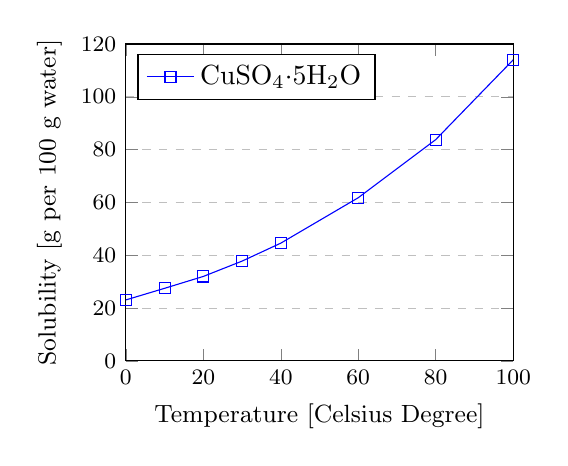
\begin{tikzpicture}
            \begin{axis}[
                    small,
                    xlabel={Temperature [Celsius Degree]},
                    ylabel={Solubility [g per 100 g water]},
                    xmin=0, xmax=100,
                    ymin=0, ymax=120,
                    xtick={0,20,40,60,80,100},
                    ytick={0,20,40,60,80,100,120},
                    legend pos=north west,
                    ymajorgrids=true,
                    grid style=dashed,
                ]
                \addplot[
                    color=blue,
                    mark=square,
                ]
                coordinates {
                        (0,23.1)(10,27.5)(20,32)(30,37.8)(40,44.6)(60,61.8)(80,83.8)(100,114)
                    };
                \legend{CuSO\(_4\cdot\)5H\(_2\)O}
            \end{axis}
        \end{tikzpicture}
        \caption{Temperature dependence of CuSO\(_4\cdot\)5H\(_2\)O solubility}\label{plot}
    \end{figure}
\end{frame}

% 谢谢收听页面
\thanksforlistening{请各位老师批评指正}

\end{document}